\documentclass[12pt]{article}
\usepackage[margin=0.75in]{geometry}
\usepackage{graphicx}
\usepackage{tikz}
\usetikzlibrary{arrows.meta, positioning, shapes.geometric}

\title{Workflow Diagram\\RoboSub LA Wailord Documentation and Control Software}
\author{CS3338 Final Project}
\date{Snapshot 4 Revision}

\begin{document}
\maketitle

\section*{High-Level Workflow}
\begin{center}
\resizebox{\textwidth}{!}{%
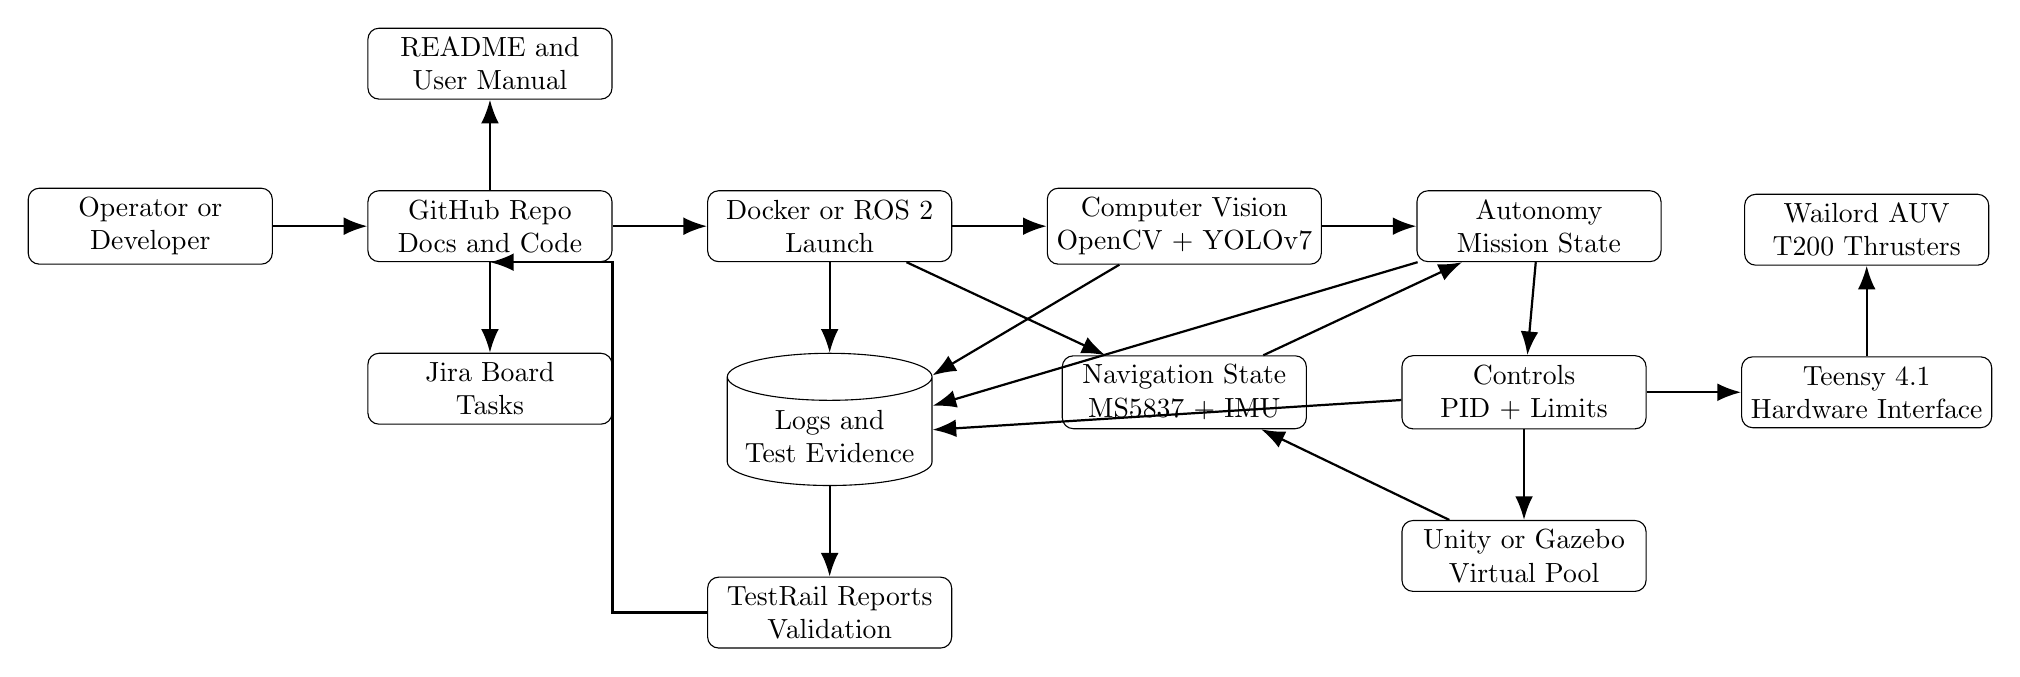
\begin{tikzpicture}[
  node distance=1.15cm and 1.2cm,
  box/.style={rectangle, draw, rounded corners, align=center, minimum width=3.1cm, minimum height=0.9cm},
  store/.style={cylinder, draw, shape border rotate=90, aspect=0.25, align=center, minimum width=2.6cm, minimum height=1.0cm},
  arrow/.style={-{Latex[length=3mm]}, thick}
]
\node[box] (user) {Operator or\\Developer};
\node[box, right=of user] (repo) {GitHub Repo\\Docs and Code};
\node[box, below=of repo] (jira) {Jira Board\\Tasks};
\node[box, above=of repo] (manual) {README and\\User Manual};
\node[box, right=of repo] (launch) {Docker or ROS 2\\Launch};
\node[box, right=of launch] (perception) {Computer Vision\\OpenCV + YOLOv7};
\node[box, below=of perception] (state) {Navigation State\\MS5837 + IMU};
\node[box, right=of perception] (autonomy) {Autonomy\\Mission State};
\node[box, right=of state] (controls) {Controls\\PID + Limits};
\node[box, right=of controls] (hardware) {Teensy 4.1\\Hardware Interface};
\node[box, above=of hardware] (physical) {Wailord AUV\\T200 Thrusters};
\node[box, below=of controls] (simulation) {Unity or Gazebo\\Virtual Pool};
\node[store, below=of launch] (logs) {Logs and\\Test Evidence};
\node[box, below=of logs] (testrail) {TestRail Reports\\Validation};

\draw[arrow] (user) -- (repo);
\draw[arrow] (repo) -- (manual);
\draw[arrow] (repo) -- (jira);
\draw[arrow] (repo) -- (launch);
\draw[arrow] (launch) -- (perception);
\draw[arrow] (launch) -- (state);
\draw[arrow] (perception) -- (autonomy);
\draw[arrow] (state) -- (autonomy);
\draw[arrow] (autonomy) -- (controls);
\draw[arrow] (controls) -- (hardware);
\draw[arrow] (hardware) -- (physical);
\draw[arrow] (controls) -- (simulation);
\draw[arrow] (simulation) -- (state);
\draw[arrow] (launch) -- (logs);
\draw[arrow] (perception) -- (logs);
\draw[arrow] (autonomy) -- (logs);
\draw[arrow] (controls) -- (logs);
\draw[arrow] (logs) -- (testrail);
\draw[arrow] (testrail.west) -- ++(-1.2,0) |- (repo.south);
\end{tikzpicture}
}
\end{center}

\section*{Workflow Explanation}
The user accesses the project through the GitHub repository, Jira board, Ascent project page, and RoboSub LA website. The repository stores the user manual, SRS, SDD, design specification, workflow diagram, snapshot objectives, and TestRail-style reports. A future runtime implementation should launch through Docker or ROS 2 Humble. The launch process starts computer vision, navigation/state estimation, autonomy, controls, Teensy hardware interface, Unity or Gazebo simulation, and logging modules.

Sensor data flows into computer vision and state estimation. Autonomy consumes those outputs and selects mission behavior. Controls converts mission goals into bounded movement commands. Commands can go to the Teensy 4.1 hardware interface and Wailord's thrusters, or to a simulated vehicle. Logs and test evidence flow into TestRail-style reports, which are stored back in the repository for review.

\end{document}
